\documentclass{standalone}
\usepackage{tikz}
\usetikzlibrary{patterns, positioning}

\begin{document}
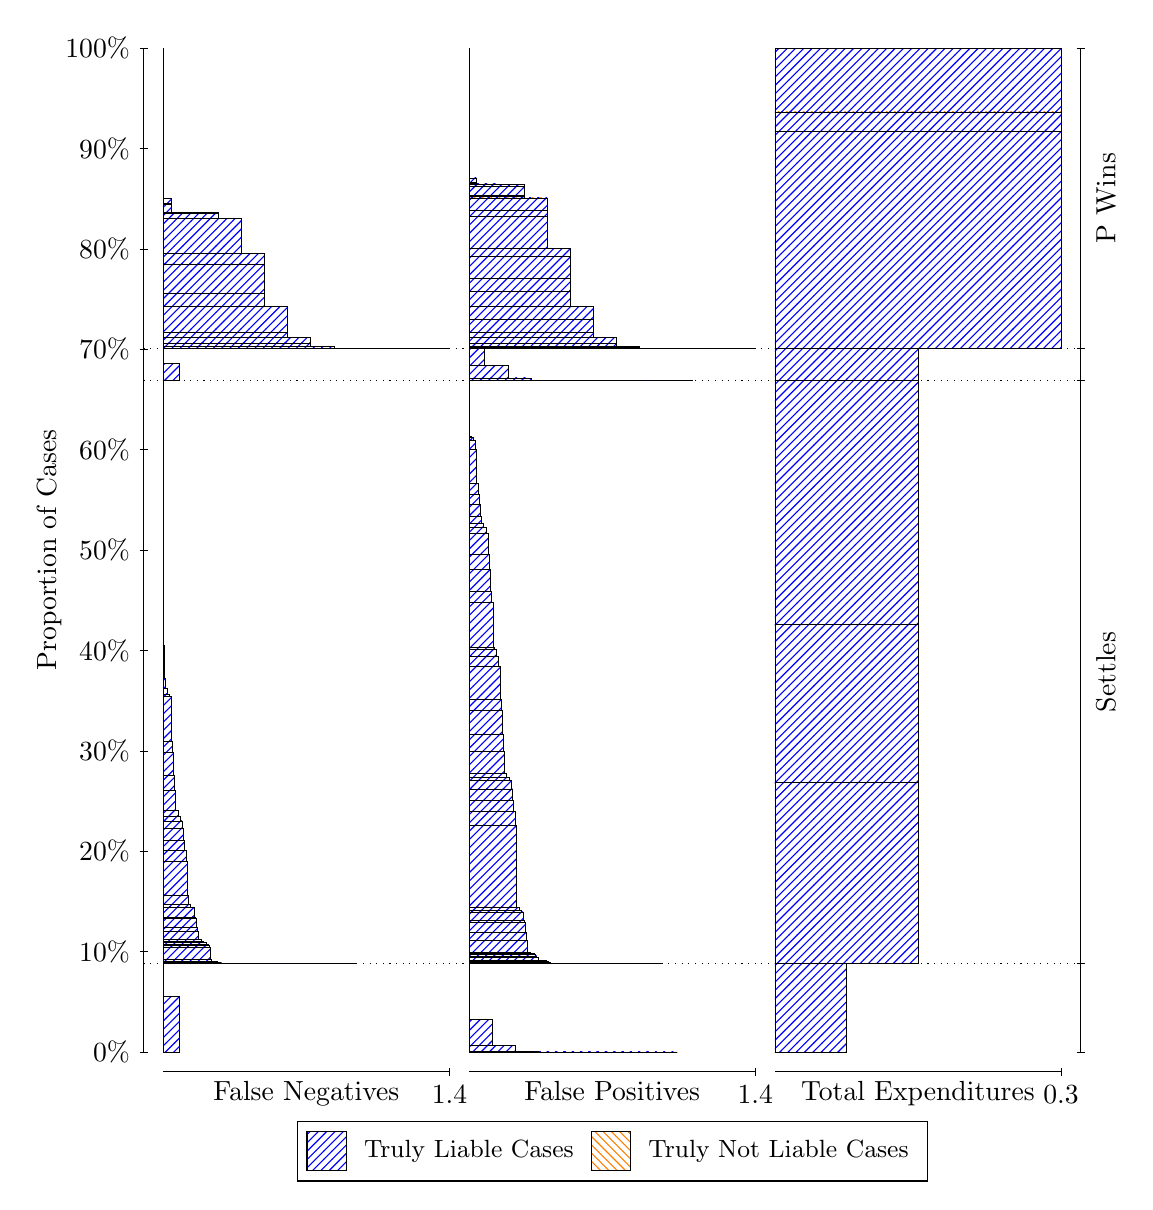
\begin{tikzpicture}
\draw[black, very thin] (1.5,1.75) -- (1.5,14.5);
\node[rotate=90, anchor=center] at (0.3, 8.125) {Proportion of Cases};
\draw[black, very thin] (1.45,1.75) -- (1.55,1.75);
\node[anchor=east] at (1.45, 1.75) {0\%};
\draw[black, very thin] (1.45,3.025) -- (1.55,3.025);
\node[anchor=east] at (1.45, 3.025) {10\%};
\draw[black, very thin] (1.45,4.3) -- (1.55,4.3);
\node[anchor=east] at (1.45, 4.3) {20\%};
\draw[black, very thin] (1.45,5.575) -- (1.55,5.575);
\node[anchor=east] at (1.45, 5.575) {30\%};
\draw[black, very thin] (1.45,6.85) -- (1.55,6.85);
\node[anchor=east] at (1.45, 6.85) {40\%};
\draw[black, very thin] (1.45,8.125) -- (1.55,8.125);
\node[anchor=east] at (1.45, 8.125) {50\%};
\draw[black, very thin] (1.45,9.4) -- (1.55,9.4);
\node[anchor=east] at (1.45, 9.4) {60\%};
\draw[black, very thin] (1.45,10.675) -- (1.55,10.675);
\node[anchor=east] at (1.45, 10.675) {70\%};
\draw[black, very thin] (1.45,11.95) -- (1.55,11.95);
\node[anchor=east] at (1.45, 11.95) {80\%};
\draw[black, very thin] (1.45,13.225) -- (1.55,13.225);
\node[anchor=east] at (1.45, 13.225) {90\%};
\draw[black, very thin] (1.45,14.5) -- (1.55,14.5);
\node[anchor=east] at (1.45, 14.5) {100\%};

\draw[black, very thin] (13.4,1.75) -- (13.4,14.5);
\draw[black, very thin] (13.35,1.75) -- (13.45,1.75);
\node[anchor=west] at (13.35, 1.75) {};
\draw[black, very thin] (13.35,2.8721) -- (13.45,2.8721);
\node[anchor=west] at (13.35, 2.8721) {};
\draw[black, very thin] (13.35,10.276) -- (13.45,10.276);
\node[anchor=west] at (13.35, 10.276) {};
\draw[black, very thin] (13.35,10.684) -- (13.45,10.684);
\node[anchor=west] at (13.35, 10.684) {};
\draw[black, very thin] (13.35,14.5) -- (13.45,14.5);
\node[anchor=west] at (13.35, 14.5) {};

\draw[black, very thin, pattern color=blue, pattern=north east lines] (1.75,1.75) rectangle (1.9482,2.4561);
\draw[black, very thin, pattern color=orange, pattern=north west lines] (1.75,2.4561) rectangle (1.75,2.4561);
\draw[black, very thin, pattern color=blue, pattern=north east lines] (1.75,2.4561) rectangle (1.75,2.8721);
\draw[black, very thin, pattern color=blue, pattern=north east lines] (1.75,2.8721) rectangle (4.1942,2.8721);
\draw[black, very thin, pattern color=blue, pattern=north east lines] (1.75,2.8721) rectangle (4.0621,2.8721);
\draw[black, very thin, pattern color=blue, pattern=north east lines] (1.75,2.8721) rectangle (3.93,2.8721);
\draw[black, very thin, pattern color=blue, pattern=north east lines] (1.75,2.8721) rectangle (3.9006,2.8721);
\draw[black, very thin, pattern color=blue, pattern=north east lines] (1.75,2.8721) rectangle (3.7979,2.8721);
\draw[black, very thin, pattern color=blue, pattern=north east lines] (1.75,2.8721) rectangle (3.7685,2.8721);
\draw[black, very thin, pattern color=blue, pattern=north east lines] (1.75,2.8721) rectangle (3.6658,2.8721);
\draw[black, very thin, pattern color=blue, pattern=north east lines] (1.75,2.8721) rectangle (3.6364,2.8721);
\draw[black, very thin, pattern color=blue, pattern=north east lines] (1.75,2.8721) rectangle (3.607,2.8721);
\draw[black, very thin, pattern color=blue, pattern=north east lines] (1.75,2.8721) rectangle (3.5336,2.8721);
\draw[black, very thin, pattern color=blue, pattern=north east lines] (1.75,2.8721) rectangle (3.5043,2.8721);
\draw[black, very thin, pattern color=blue, pattern=north east lines] (1.75,2.8721) rectangle (3.4749,2.8721);
\draw[black, very thin, pattern color=blue, pattern=north east lines] (1.75,2.8721) rectangle (3.4015,2.8721);
\draw[black, very thin, pattern color=blue, pattern=north east lines] (1.75,2.8721) rectangle (3.3722,2.8721);
\draw[black, very thin, pattern color=blue, pattern=north east lines] (1.75,2.8721) rectangle (3.3428,2.8721);
\draw[black, very thin, pattern color=blue, pattern=north east lines] (1.75,2.8721) rectangle (3.3134,2.8721);
\draw[black, very thin, pattern color=blue, pattern=north east lines] (1.75,2.8721) rectangle (3.2694,2.8721);
\draw[black, very thin, pattern color=blue, pattern=north east lines] (1.75,2.8721) rectangle (3.24,2.8721);
\draw[black, very thin, pattern color=blue, pattern=north east lines] (1.75,2.8721) rectangle (3.2107,2.8721);
\draw[black, very thin, pattern color=blue, pattern=north east lines] (1.75,2.8721) rectangle (3.1813,2.8721);
\draw[black, very thin, pattern color=blue, pattern=north east lines] (1.75,2.8721) rectangle (3.1373,2.8721);
\draw[black, very thin, pattern color=blue, pattern=north east lines] (1.75,2.8721) rectangle (3.1079,2.8721);
\draw[black, very thin, pattern color=blue, pattern=north east lines] (1.75,2.8721) rectangle (3.0786,2.8721);
\draw[black, very thin, pattern color=blue, pattern=north east lines] (1.75,2.8721) rectangle (3.0492,2.8721);
\draw[black, very thin, pattern color=blue, pattern=north east lines] (1.75,2.8721) rectangle (3.0198,2.8721);
\draw[black, very thin, pattern color=blue, pattern=north east lines] (1.75,2.8721) rectangle (3.0052,2.8721);
\draw[black, very thin, pattern color=blue, pattern=north east lines] (1.75,2.8721) rectangle (2.9758,2.8721);
\draw[black, very thin, pattern color=blue, pattern=north east lines] (1.75,2.8721) rectangle (2.9464,2.8721);
\draw[black, very thin, pattern color=blue, pattern=north east lines] (1.75,2.8721) rectangle (2.9171,2.8721);
\draw[black, very thin, pattern color=blue, pattern=north east lines] (1.75,2.8721) rectangle (2.8877,2.8721);
\draw[black, very thin, pattern color=blue, pattern=north east lines] (1.75,2.8721) rectangle (2.873,2.8721);
\draw[black, very thin, pattern color=blue, pattern=north east lines] (1.75,2.8721) rectangle (2.8437,2.8721);
\draw[black, very thin, pattern color=blue, pattern=north east lines] (1.75,2.8721) rectangle (2.8143,2.8721);
\draw[black, very thin, pattern color=blue, pattern=north east lines] (1.75,2.8721) rectangle (2.7849,2.8722);
\draw[black, very thin, pattern color=blue, pattern=north east lines] (1.75,2.8722) rectangle (2.7556,2.8722);
\draw[black, very thin, pattern color=blue, pattern=north east lines] (1.75,2.8722) rectangle (2.7409,2.8722);
\draw[black, very thin, pattern color=blue, pattern=north east lines] (1.75,2.8722) rectangle (2.7262,2.8723);
\draw[black, very thin, pattern color=blue, pattern=north east lines] (1.75,2.8723) rectangle (2.7115,2.8723);
\draw[black, very thin, pattern color=blue, pattern=north east lines] (1.75,2.8723) rectangle (2.6822,2.8723);
\draw[black, very thin, pattern color=blue, pattern=north east lines] (1.75,2.8723) rectangle (2.6528,2.8728);
\draw[black, very thin, pattern color=blue, pattern=north east lines] (1.75,2.8728) rectangle (2.6235,2.8733);
\draw[black, very thin, pattern color=blue, pattern=north east lines] (1.75,2.8733) rectangle (2.6088,2.8736);
\draw[black, very thin, pattern color=blue, pattern=north east lines] (1.75,2.8736) rectangle (2.5941,2.8741);
\draw[black, very thin, pattern color=blue, pattern=north east lines] (1.75,2.8741) rectangle (2.5794,2.8742);
\draw[black, very thin, pattern color=blue, pattern=north east lines] (1.75,2.8742) rectangle (2.5501,2.8744);
\draw[black, very thin, pattern color=blue, pattern=north east lines] (1.75,2.8744) rectangle (2.5207,2.8758);
\draw[black, very thin, pattern color=blue, pattern=north east lines] (1.75,2.8758) rectangle (2.4913,2.8823);
\draw[black, very thin, pattern color=blue, pattern=north east lines] (1.75,2.8823) rectangle (2.4767,2.8871);
\draw[black, very thin, pattern color=blue, pattern=north east lines] (1.75,2.8871) rectangle (2.462,2.8937);
\draw[black, very thin, pattern color=blue, pattern=north east lines] (1.75,2.8937) rectangle (2.4473,2.8943);
\draw[black, very thin, pattern color=blue, pattern=north east lines] (1.75,2.8943) rectangle (2.4326,2.8999);
\draw[black, very thin, pattern color=blue, pattern=north east lines] (1.75,2.8999) rectangle (2.4179,2.9006);
\draw[black, very thin, pattern color=blue, pattern=north east lines] (1.75,2.9006) rectangle (2.3886,2.9026);
\draw[black, very thin, pattern color=blue, pattern=north east lines] (1.75,2.9026) rectangle (2.3592,2.9215);
\draw[black, very thin, pattern color=blue, pattern=north east lines] (1.75,2.9215) rectangle (2.3445,3.086);
\draw[black, very thin, pattern color=blue, pattern=north east lines] (1.75,3.086) rectangle (2.3299,3.1075);
\draw[black, very thin, pattern color=blue, pattern=north east lines] (1.75,3.1075) rectangle (2.3152,3.1185);
\draw[black, very thin, pattern color=blue, pattern=north east lines] (1.75,3.1185) rectangle (2.3005,3.139);
\draw[black, very thin, pattern color=blue, pattern=north east lines] (1.75,3.139) rectangle (2.2858,3.1455);
\draw[black, very thin, pattern color=blue, pattern=north east lines] (1.75,3.1455) rectangle (2.2565,3.154);
\draw[black, very thin, pattern color=blue, pattern=north east lines] (1.75,3.154) rectangle (2.2271,3.1792);
\draw[black, very thin, pattern color=blue, pattern=north east lines] (1.75,3.1792) rectangle (2.1977,3.2826);
\draw[black, very thin, pattern color=blue, pattern=north east lines] (1.75,3.2826) rectangle (2.1831,3.338);
\draw[black, very thin, pattern color=blue, pattern=north east lines] (1.75,3.338) rectangle (2.1684,3.4447);
\draw[black, very thin, pattern color=blue, pattern=north east lines] (1.75,3.4447) rectangle (2.1537,3.4649);
\draw[black, very thin, pattern color=blue, pattern=north east lines] (1.75,3.4649) rectangle (2.139,3.5829);
\draw[black, very thin, pattern color=blue, pattern=north east lines] (1.75,3.5829) rectangle (2.1243,3.594);
\draw[black, very thin, pattern color=blue, pattern=north east lines] (1.75,3.594) rectangle (2.095,3.6254);
\draw[black, very thin, pattern color=blue, pattern=north east lines] (1.75,3.6254) rectangle (2.0656,3.7463);
\draw[black, very thin, pattern color=blue, pattern=north east lines] (1.75,3.7463) rectangle (2.0509,4.1752);
\draw[black, very thin, pattern color=blue, pattern=north east lines] (1.75,4.1752) rectangle (2.0363,4.3127);
\draw[black, very thin, pattern color=blue, pattern=north east lines] (1.75,4.3127) rectangle (2.0216,4.4404);
\draw[black, very thin, pattern color=blue, pattern=north east lines] (1.75,4.4404) rectangle (2.0069,4.5899);
\draw[black, very thin, pattern color=blue, pattern=north east lines] (1.75,4.5899) rectangle (1.9922,4.6845);
\draw[black, very thin, pattern color=blue, pattern=north east lines] (1.75,4.6845) rectangle (1.9629,4.7387);
\draw[black, very thin, pattern color=blue, pattern=north east lines] (1.75,4.7387) rectangle (1.9335,4.8138);
\draw[black, very thin, pattern color=blue, pattern=north east lines] (1.75,4.8138) rectangle (1.9041,5.0745);
\draw[black, very thin, pattern color=blue, pattern=north east lines] (1.75,5.0745) rectangle (1.8895,5.2694);
\draw[black, very thin, pattern color=blue, pattern=north east lines] (1.75,5.2694) rectangle (1.8748,5.5519);
\draw[black, very thin, pattern color=blue, pattern=north east lines] (1.75,5.5519) rectangle (1.8601,5.6908);
\draw[black, very thin, pattern color=blue, pattern=north east lines] (1.75,5.6908) rectangle (1.8454,6.2621);
\draw[black, very thin, pattern color=blue, pattern=north east lines] (1.75,6.2621) rectangle (1.8307,6.2893);
\draw[black, very thin, pattern color=blue, pattern=north east lines] (1.75,6.2893) rectangle (1.8014,6.3686);
\draw[black, very thin, pattern color=blue, pattern=north east lines] (1.75,6.3686) rectangle (1.772,6.4941);
\draw[black, very thin, pattern color=blue, pattern=north east lines] (1.75,6.4941) rectangle (1.7573,6.9186);
\draw[black, very thin, pattern color=orange, pattern=north west lines] (1.75,6.9186) rectangle (1.75,6.9186);
\draw[black, very thin, pattern color=blue, pattern=north east lines] (1.75,6.9186) rectangle (1.75,10.276);
\draw[black, very thin, pattern color=blue, pattern=north east lines] (1.75,10.276) rectangle (1.9482,10.492);
\draw[black, very thin, pattern color=orange, pattern=north west lines] (1.75,10.492) rectangle (1.75,10.492);
\draw[black, very thin, pattern color=blue, pattern=north east lines] (1.75,10.492) rectangle (1.75,10.684);
\draw[black, very thin, pattern color=blue, pattern=north east lines] (1.75,10.684) rectangle (5.3833,10.684);
\draw[black, very thin, pattern color=blue, pattern=north east lines] (1.75,10.684) rectangle (5.0897,10.684);
\draw[black, very thin, pattern color=blue, pattern=north east lines] (1.75,10.684) rectangle (4.7961,10.684);
\draw[black, very thin, pattern color=blue, pattern=north east lines] (1.75,10.684) rectangle (4.5025,10.684);
\draw[black, very thin, pattern color=blue, pattern=north east lines] (1.75,10.684) rectangle (4.5025,10.684);
\draw[black, very thin, pattern color=blue, pattern=north east lines] (1.75,10.684) rectangle (4.2089,10.687);
\draw[black, very thin, pattern color=blue, pattern=north east lines] (1.75,10.687) rectangle (3.9153,10.709);
\draw[black, very thin, pattern color=blue, pattern=north east lines] (1.75,10.709) rectangle (3.6217,10.755);
\draw[black, very thin, pattern color=blue, pattern=north east lines] (1.75,10.755) rectangle (3.6217,10.828);
\draw[black, very thin, pattern color=blue, pattern=north east lines] (1.75,10.828) rectangle (3.607,10.828);
\draw[black, very thin, pattern color=blue, pattern=north east lines] (1.75,10.828) rectangle (3.3281,10.885);
\draw[black, very thin, pattern color=blue, pattern=north east lines] (1.75,10.885) rectangle (3.3281,11.222);
\draw[black, very thin, pattern color=blue, pattern=north east lines] (1.75,11.222) rectangle (3.3134,11.222);
\draw[black, very thin, pattern color=blue, pattern=north east lines] (1.75,11.222) rectangle (3.0345,11.383);
\draw[black, very thin, pattern color=blue, pattern=north east lines] (1.75,11.383) rectangle (3.0345,11.76);
\draw[black, very thin, pattern color=blue, pattern=north east lines] (1.75,11.76) rectangle (3.0345,11.892);
\draw[black, very thin, pattern color=blue, pattern=north east lines] (1.75,11.892) rectangle (3.0198,11.892);
\draw[black, very thin, pattern color=blue, pattern=north east lines] (1.75,11.892) rectangle (3.0198,11.892);
\draw[black, very thin, pattern color=blue, pattern=north east lines] (1.75,11.892) rectangle (2.7409,12.334);
\draw[black, very thin, pattern color=blue, pattern=north east lines] (1.75,12.334) rectangle (2.7262,12.334);
\draw[black, very thin, pattern color=blue, pattern=north east lines] (1.75,12.334) rectangle (2.4473,12.338);
\draw[black, very thin, pattern color=blue, pattern=north east lines] (1.75,12.338) rectangle (2.4473,12.403);
\draw[black, very thin, pattern color=blue, pattern=north east lines] (1.75,12.403) rectangle (2.4473,12.41);
\draw[black, very thin, pattern color=blue, pattern=north east lines] (1.75,12.41) rectangle (2.4326,12.41);
\draw[black, very thin, pattern color=blue, pattern=north east lines] (1.75,12.41) rectangle (2.4326,12.41);
\draw[black, very thin, pattern color=blue, pattern=north east lines] (1.75,12.41) rectangle (2.1537,12.411);
\draw[black, very thin, pattern color=blue, pattern=north east lines] (1.75,12.411) rectangle (2.1537,12.411);
\draw[black, very thin, pattern color=blue, pattern=north east lines] (1.75,12.411) rectangle (2.139,12.417);
\draw[black, very thin, pattern color=blue, pattern=north east lines] (1.75,12.417) rectangle (1.8601,12.417);
\draw[black, very thin, pattern color=blue, pattern=north east lines] (1.75,12.417) rectangle (1.8601,12.417);
\draw[black, very thin, pattern color=blue, pattern=north east lines] (1.75,12.417) rectangle (1.8454,12.513);
\draw[black, very thin, pattern color=blue, pattern=north east lines] (1.75,12.513) rectangle (1.8454,12.53);
\draw[black, very thin, pattern color=blue, pattern=north east lines] (1.75,12.53) rectangle (1.8454,12.586);
\draw[black, very thin, pattern color=orange, pattern=north west lines] (1.75,12.586) rectangle (1.75,12.586);
\draw[black, very thin, pattern color=blue, pattern=north east lines] (1.75,12.586) rectangle (1.75,14.5);
\draw[black, very thin, pattern color=orange, pattern=north west lines] (5.6333,1.75) rectangle (8.2758,1.75);
\draw[black, very thin, pattern color=blue, pattern=north east lines] (5.6333,1.75) rectangle (8.2758,1.75);
\draw[black, very thin, pattern color=blue, pattern=north east lines] (5.6333,1.75) rectangle (7.9822,1.75);
\draw[black, very thin, pattern color=blue, pattern=north east lines] (5.6333,1.75) rectangle (7.6886,1.75);
\draw[black, very thin, pattern color=blue, pattern=north east lines] (5.6333,1.75) rectangle (7.3949,1.75);
\draw[black, very thin, pattern color=blue, pattern=north east lines] (5.6333,1.75) rectangle (7.1013,1.75);
\draw[black, very thin, pattern color=blue, pattern=north east lines] (5.6333,1.75) rectangle (6.8077,1.7503);
\draw[black, very thin, pattern color=blue, pattern=north east lines] (5.6333,1.7503) rectangle (6.5141,1.7579);
\draw[black, very thin, pattern color=blue, pattern=north east lines] (5.6333,1.7579) rectangle (6.2205,1.8357);
\draw[black, very thin, pattern color=blue, pattern=north east lines] (5.6333,1.8357) rectangle (5.9269,2.166);
\draw[black, very thin, pattern color=blue, pattern=north east lines] (5.6333,2.166) rectangle (5.6333,2.8721);
\draw[black, very thin, pattern color=orange, pattern=north west lines] (5.6333,2.8721) rectangle (8.0776,2.8721);
\draw[black, very thin, pattern color=blue, pattern=north east lines] (5.6333,2.8721) rectangle (8.0776,2.8721);
\draw[black, very thin, pattern color=orange, pattern=north west lines] (5.6333,2.8721) rectangle (7.9455,2.8721);
\draw[black, very thin, pattern color=blue, pattern=north east lines] (5.6333,2.8721) rectangle (7.9455,2.8721);
\draw[black, very thin, pattern color=orange, pattern=north west lines] (5.6333,2.8721) rectangle (7.8133,2.8721);
\draw[black, very thin, pattern color=blue, pattern=north east lines] (5.6333,2.8721) rectangle (7.8133,2.8721);
\draw[black, very thin, pattern color=blue, pattern=north east lines] (5.6333,2.8721) rectangle (7.784,2.8721);
\draw[black, very thin, pattern color=orange, pattern=north west lines] (5.6333,2.8721) rectangle (7.6812,2.8721);
\draw[black, very thin, pattern color=blue, pattern=north east lines] (5.6333,2.8721) rectangle (7.6812,2.8721);
\draw[black, very thin, pattern color=blue, pattern=north east lines] (5.6333,2.8721) rectangle (7.6519,2.8721);
\draw[black, very thin, pattern color=orange, pattern=north west lines] (5.6333,2.8721) rectangle (7.5491,2.8721);
\draw[black, very thin, pattern color=blue, pattern=north east lines] (5.6333,2.8721) rectangle (7.5491,2.8721);
\draw[black, very thin, pattern color=blue, pattern=north east lines] (5.6333,2.8721) rectangle (7.5197,2.8721);
\draw[black, very thin, pattern color=blue, pattern=north east lines] (5.6333,2.8721) rectangle (7.4904,2.8721);
\draw[black, very thin, pattern color=orange, pattern=north west lines] (5.6333,2.8721) rectangle (7.417,2.8721);
\draw[black, very thin, pattern color=blue, pattern=north east lines] (5.6333,2.8721) rectangle (7.417,2.8721);
\draw[black, very thin, pattern color=blue, pattern=north east lines] (5.6333,2.8721) rectangle (7.3876,2.8721);
\draw[black, very thin, pattern color=blue, pattern=north east lines] (5.6333,2.8721) rectangle (7.3582,2.8721);
\draw[black, very thin, pattern color=orange, pattern=north west lines] (5.6333,2.8721) rectangle (7.2848,2.8721);
\draw[black, very thin, pattern color=blue, pattern=north east lines] (5.6333,2.8721) rectangle (7.2848,2.8721);
\draw[black, very thin, pattern color=blue, pattern=north east lines] (5.6333,2.8721) rectangle (7.2555,2.8721);
\draw[black, very thin, pattern color=blue, pattern=north east lines] (5.6333,2.8721) rectangle (7.2261,2.8721);
\draw[black, very thin, pattern color=blue, pattern=north east lines] (5.6333,2.8721) rectangle (7.1968,2.8721);
\draw[black, very thin, pattern color=orange, pattern=north west lines] (5.6333,2.8721) rectangle (7.1527,2.8721);
\draw[black, very thin, pattern color=blue, pattern=north east lines] (5.6333,2.8721) rectangle (7.1527,2.8721);
\draw[black, very thin, pattern color=blue, pattern=north east lines] (5.6333,2.8721) rectangle (7.1234,2.8721);
\draw[black, very thin, pattern color=blue, pattern=north east lines] (5.6333,2.8721) rectangle (7.094,2.8721);
\draw[black, very thin, pattern color=blue, pattern=north east lines] (5.6333,2.8721) rectangle (7.0646,2.8721);
\draw[black, very thin, pattern color=orange, pattern=north west lines] (5.6333,2.8721) rectangle (7.0206,2.8721);
\draw[black, very thin, pattern color=blue, pattern=north east lines] (5.6333,2.8721) rectangle (7.0206,2.8721);
\draw[black, very thin, pattern color=blue, pattern=north east lines] (5.6333,2.8721) rectangle (6.9912,2.8721);
\draw[black, very thin, pattern color=blue, pattern=north east lines] (5.6333,2.8721) rectangle (6.9619,2.8725);
\draw[black, very thin, pattern color=blue, pattern=north east lines] (5.6333,2.8725) rectangle (6.9325,2.8726);
\draw[black, very thin, pattern color=blue, pattern=north east lines] (5.6333,2.8726) rectangle (6.9032,2.8726);
\draw[black, very thin, pattern color=orange, pattern=north west lines] (5.6333,2.8726) rectangle (6.8885,2.8726);
\draw[black, very thin, pattern color=blue, pattern=north east lines] (5.6333,2.8726) rectangle (6.8885,2.8726);
\draw[black, very thin, pattern color=blue, pattern=north east lines] (5.6333,2.8726) rectangle (6.8591,2.8727);
\draw[black, very thin, pattern color=blue, pattern=north east lines] (5.6333,2.8727) rectangle (6.8298,2.8727);
\draw[black, very thin, pattern color=blue, pattern=north east lines] (5.6333,2.8727) rectangle (6.8004,2.8744);
\draw[black, very thin, pattern color=blue, pattern=north east lines] (5.6333,2.8744) rectangle (6.771,2.8749);
\draw[black, very thin, pattern color=orange, pattern=north west lines] (5.6333,2.8749) rectangle (6.7564,2.8749);
\draw[black, very thin, pattern color=blue, pattern=north east lines] (5.6333,2.8749) rectangle (6.7564,2.8751);
\draw[black, very thin, pattern color=blue, pattern=north east lines] (5.6333,2.8751) rectangle (6.727,2.8752);
\draw[black, very thin, pattern color=blue, pattern=north east lines] (5.6333,2.8752) rectangle (6.6976,2.8754);
\draw[black, very thin, pattern color=blue, pattern=north east lines] (5.6333,2.8754) rectangle (6.6683,2.8932);
\draw[black, very thin, pattern color=blue, pattern=north east lines] (5.6333,2.8932) rectangle (6.6389,2.9019);
\draw[black, very thin, pattern color=orange, pattern=north west lines] (5.6333,2.9019) rectangle (6.6242,2.9019);
\draw[black, very thin, pattern color=blue, pattern=north east lines] (5.6333,2.9019) rectangle (6.6242,2.9034);
\draw[black, very thin, pattern color=blue, pattern=north east lines] (5.6333,2.9034) rectangle (6.6096,2.9088);
\draw[black, very thin, pattern color=blue, pattern=north east lines] (5.6333,2.9088) rectangle (6.5949,2.9096);
\draw[black, very thin, pattern color=blue, pattern=north east lines] (5.6333,2.9096) rectangle (6.5655,2.9116);
\draw[black, very thin, pattern color=blue, pattern=north east lines] (5.6333,2.9116) rectangle (6.5362,2.9123);
\draw[black, very thin, pattern color=blue, pattern=north east lines] (5.6333,2.9123) rectangle (6.5068,2.9518);
\draw[black, very thin, pattern color=orange, pattern=north west lines] (5.6333,2.9518) rectangle (6.4921,2.9518);
\draw[black, very thin, pattern color=blue, pattern=north east lines] (5.6333,2.9518) rectangle (6.4921,2.9714);
\draw[black, very thin, pattern color=blue, pattern=north east lines] (5.6333,2.9714) rectangle (6.4774,2.9919);
\draw[black, very thin, pattern color=blue, pattern=north east lines] (5.6333,2.9919) rectangle (6.4628,2.9996);
\draw[black, very thin, pattern color=blue, pattern=north east lines] (5.6333,2.9996) rectangle (6.4334,3.0041);
\draw[black, very thin, pattern color=blue, pattern=north east lines] (5.6333,3.0041) rectangle (6.404,3.0127);
\draw[black, very thin, pattern color=blue, pattern=north east lines] (5.6333,3.0127) rectangle (6.3747,3.1711);
\draw[black, very thin, pattern color=orange, pattern=north west lines] (5.6333,3.1711) rectangle (6.36,3.1711);
\draw[black, very thin, pattern color=blue, pattern=north east lines] (5.6333,3.1711) rectangle (6.36,3.272);
\draw[black, very thin, pattern color=blue, pattern=north east lines] (5.6333,3.272) rectangle (6.3453,3.3934);
\draw[black, very thin, pattern color=blue, pattern=north east lines] (5.6333,3.3934) rectangle (6.3306,3.4208);
\draw[black, very thin, pattern color=blue, pattern=north east lines] (5.6333,3.4208) rectangle (6.316,3.5279);
\draw[black, very thin, pattern color=blue, pattern=north east lines] (5.6333,3.5279) rectangle (6.3013,3.55);
\draw[black, very thin, pattern color=blue, pattern=north east lines] (5.6333,3.55) rectangle (6.2719,3.5815);
\draw[black, very thin, pattern color=blue, pattern=north east lines] (5.6333,3.5815) rectangle (6.2426,3.5922);
\draw[black, very thin, pattern color=orange, pattern=north west lines] (5.6333,3.5922) rectangle (6.2279,3.5922);
\draw[black, very thin, pattern color=blue, pattern=north east lines] (5.6333,3.5922) rectangle (6.2279,4.6327);
\draw[black, very thin, pattern color=blue, pattern=north east lines] (5.6333,4.6327) rectangle (6.2132,4.8031);
\draw[black, very thin, pattern color=blue, pattern=north east lines] (5.6333,4.8031) rectangle (6.1985,4.9434);
\draw[black, very thin, pattern color=blue, pattern=north east lines] (5.6333,4.9434) rectangle (6.1838,5.0911);
\draw[black, very thin, pattern color=blue, pattern=north east lines] (5.6333,5.0911) rectangle (6.1692,5.197);
\draw[black, very thin, pattern color=blue, pattern=north east lines] (5.6333,5.197) rectangle (6.1398,5.2387);
\draw[black, very thin, pattern color=blue, pattern=north east lines] (5.6333,5.2387) rectangle (6.1104,5.2929);
\draw[black, very thin, pattern color=blue, pattern=north east lines] (5.6333,5.2929) rectangle (6.0811,5.569);
\draw[black, very thin, pattern color=blue, pattern=north east lines] (5.6333,5.569) rectangle (6.0664,5.79);
\draw[black, very thin, pattern color=blue, pattern=north east lines] (5.6333,5.79) rectangle (6.0517,6.0868);
\draw[black, very thin, pattern color=blue, pattern=north east lines] (5.6333,6.0868) rectangle (6.037,6.2296);
\draw[black, very thin, pattern color=blue, pattern=north east lines] (5.6333,6.2296) rectangle (6.0224,6.6541);
\draw[black, very thin, pattern color=blue, pattern=north east lines] (5.6333,6.6541) rectangle (6.0077,6.7796);
\draw[black, very thin, pattern color=blue, pattern=north east lines] (5.6333,6.7796) rectangle (5.9783,6.8588);
\draw[black, very thin, pattern color=blue, pattern=north east lines] (5.6333,6.8588) rectangle (5.949,6.8861);
\draw[black, very thin, pattern color=blue, pattern=north east lines] (5.6333,6.8861) rectangle (5.9343,7.4574);
\draw[black, very thin, pattern color=blue, pattern=north east lines] (5.6333,7.4574) rectangle (5.9196,7.5962);
\draw[black, very thin, pattern color=blue, pattern=north east lines] (5.6333,7.5962) rectangle (5.9049,7.8787);
\draw[black, very thin, pattern color=blue, pattern=north east lines] (5.6333,7.8787) rectangle (5.8902,8.0737);
\draw[black, very thin, pattern color=blue, pattern=north east lines] (5.6333,8.0737) rectangle (5.8756,8.3344);
\draw[black, very thin, pattern color=blue, pattern=north east lines] (5.6333,8.3344) rectangle (5.8462,8.4095);
\draw[black, very thin, pattern color=blue, pattern=north east lines] (5.6333,8.4095) rectangle (5.8168,8.4637);
\draw[black, very thin, pattern color=blue, pattern=north east lines] (5.6333,8.4637) rectangle (5.7875,8.5583);
\draw[black, very thin, pattern color=blue, pattern=north east lines] (5.6333,8.5583) rectangle (5.7728,8.7077);
\draw[black, very thin, pattern color=blue, pattern=north east lines] (5.6333,8.7077) rectangle (5.7581,8.8354);
\draw[black, very thin, pattern color=blue, pattern=north east lines] (5.6333,8.8354) rectangle (5.7434,8.973);
\draw[black, very thin, pattern color=blue, pattern=north east lines] (5.6333,8.973) rectangle (5.7288,9.4019);
\draw[black, very thin, pattern color=blue, pattern=north east lines] (5.6333,9.4019) rectangle (5.7141,9.5227);
\draw[black, very thin, pattern color=blue, pattern=north east lines] (5.6333,9.5227) rectangle (5.6847,9.5542);
\draw[black, very thin, pattern color=blue, pattern=north east lines] (5.6333,9.5542) rectangle (5.6554,9.5653);
\draw[black, very thin, pattern color=blue, pattern=north east lines] (5.6333,9.5653) rectangle (5.6407,9.6833);
\draw[black, very thin, pattern color=blue, pattern=north east lines] (5.6333,9.6833) rectangle (5.6333,10.276);
\draw[black, very thin, pattern color=orange, pattern=north west lines] (5.6333,10.276) rectangle (8.4739,10.276);
\draw[black, very thin, pattern color=blue, pattern=north east lines] (5.6333,10.276) rectangle (8.4739,10.276);
\draw[black, very thin, pattern color=blue, pattern=north east lines] (5.6333,10.276) rectangle (8.1803,10.276);
\draw[black, very thin, pattern color=blue, pattern=north east lines] (5.6333,10.276) rectangle (7.8867,10.276);
\draw[black, very thin, pattern color=blue, pattern=north east lines] (5.6333,10.276) rectangle (7.5931,10.276);
\draw[black, very thin, pattern color=blue, pattern=north east lines] (5.6333,10.276) rectangle (7.2995,10.276);
\draw[black, very thin, pattern color=blue, pattern=north east lines] (5.6333,10.276) rectangle (7.0059,10.276);
\draw[black, very thin, pattern color=blue, pattern=north east lines] (5.6333,10.276) rectangle (6.7123,10.278);
\draw[black, very thin, pattern color=blue, pattern=north east lines] (5.6333,10.278) rectangle (6.4187,10.312);
\draw[black, very thin, pattern color=blue, pattern=north east lines] (5.6333,10.312) rectangle (6.1251,10.468);
\draw[black, very thin, pattern color=blue, pattern=north east lines] (5.6333,10.468) rectangle (5.8315,10.684);
\draw[black, very thin, pattern color=orange, pattern=north west lines] (5.6333,10.684) rectangle (9.2667,10.684);
\draw[black, very thin, pattern color=blue, pattern=north east lines] (5.6333,10.684) rectangle (9.2667,10.684);
\draw[black, very thin, pattern color=orange, pattern=north west lines] (5.6333,10.684) rectangle (8.9731,10.684);
\draw[black, very thin, pattern color=blue, pattern=north east lines] (5.6333,10.684) rectangle (8.9731,10.684);
\draw[black, very thin, pattern color=orange, pattern=north west lines] (5.6333,10.684) rectangle (8.6795,10.684);
\draw[black, very thin, pattern color=blue, pattern=north east lines] (5.6333,10.684) rectangle (8.6795,10.684);
\draw[black, very thin, pattern color=blue, pattern=north east lines] (5.6333,10.684) rectangle (8.3859,10.684);
\draw[black, very thin, pattern color=orange, pattern=north west lines] (5.6333,10.684) rectangle (8.3859,10.684);
\draw[black, very thin, pattern color=blue, pattern=north east lines] (5.6333,10.684) rectangle (8.3859,10.684);
\draw[black, very thin, pattern color=orange, pattern=north west lines] (5.6333,10.684) rectangle (8.0923,10.684);
\draw[black, very thin, pattern color=blue, pattern=north east lines] (5.6333,10.684) rectangle (8.0923,10.686);
\draw[black, very thin, pattern color=blue, pattern=north east lines] (5.6333,10.686) rectangle (8.0923,10.687);
\draw[black, very thin, pattern color=blue, pattern=north east lines] (5.6333,10.687) rectangle (8.0923,10.687);
\draw[black, very thin, pattern color=orange, pattern=north west lines] (5.6333,10.687) rectangle (7.7987,10.687);
\draw[black, very thin, pattern color=blue, pattern=north east lines] (5.6333,10.687) rectangle (7.7987,10.705);
\draw[black, very thin, pattern color=blue, pattern=north east lines] (5.6333,10.705) rectangle (7.7987,10.709);
\draw[black, very thin, pattern color=blue, pattern=north east lines] (5.6333,10.709) rectangle (7.5051,10.745);
\draw[black, very thin, pattern color=orange, pattern=north west lines] (5.6333,10.745) rectangle (7.5051,10.745);
\draw[black, very thin, pattern color=blue, pattern=north east lines] (5.6333,10.745) rectangle (7.5051,10.827);
\draw[black, very thin, pattern color=orange, pattern=north west lines] (5.6333,10.827) rectangle (7.4904,10.827);
\draw[black, very thin, pattern color=blue, pattern=north east lines] (5.6333,10.827) rectangle (7.4904,10.827);
\draw[black, very thin, pattern color=blue, pattern=north east lines] (5.6333,10.827) rectangle (7.2114,10.885);
\draw[black, very thin, pattern color=orange, pattern=north west lines] (5.6333,10.885) rectangle (7.2114,10.885);
\draw[black, very thin, pattern color=blue, pattern=north east lines] (5.6333,10.885) rectangle (7.2114,11.053);
\draw[black, very thin, pattern color=blue, pattern=north east lines] (5.6333,11.053) rectangle (7.2114,11.216);
\draw[black, very thin, pattern color=blue, pattern=north east lines] (5.6333,11.216) rectangle (7.1968,11.216);
\draw[black, very thin, pattern color=orange, pattern=north west lines] (5.6333,11.216) rectangle (7.1968,11.216);
\draw[black, very thin, pattern color=blue, pattern=north east lines] (5.6333,11.216) rectangle (7.1968,11.216);
\draw[black, very thin, pattern color=blue, pattern=north east lines] (5.6333,11.216) rectangle (6.9178,11.411);
\draw[black, very thin, pattern color=blue, pattern=north east lines] (5.6333,11.411) rectangle (6.9178,11.576);
\draw[black, very thin, pattern color=blue, pattern=north east lines] (5.6333,11.576) rectangle (6.9178,11.85);
\draw[black, very thin, pattern color=blue, pattern=north east lines] (5.6333,11.85) rectangle (6.9178,11.955);
\draw[black, very thin, pattern color=orange, pattern=north west lines] (5.6333,11.955) rectangle (6.9032,11.955);
\draw[black, very thin, pattern color=blue, pattern=north east lines] (5.6333,11.955) rectangle (6.9032,11.955);
\draw[black, very thin, pattern color=blue, pattern=north east lines] (5.6333,11.955) rectangle (6.9032,11.955);
\draw[black, very thin, pattern color=blue, pattern=north east lines] (5.6333,11.955) rectangle (6.6242,12.362);
\draw[black, very thin, pattern color=blue, pattern=north east lines] (5.6333,12.362) rectangle (6.6242,12.439);
\draw[black, very thin, pattern color=blue, pattern=north east lines] (5.6333,12.439) rectangle (6.6242,12.598);
\draw[black, very thin, pattern color=blue, pattern=north east lines] (5.6333,12.598) rectangle (6.6096,12.598);
\draw[black, very thin, pattern color=orange, pattern=north west lines] (5.6333,12.598) rectangle (6.6096,12.598);
\draw[black, very thin, pattern color=blue, pattern=north east lines] (5.6333,12.598) rectangle (6.6096,12.598);
\draw[black, very thin, pattern color=blue, pattern=north east lines] (5.6333,12.598) rectangle (6.3306,12.616);
\draw[black, very thin, pattern color=blue, pattern=north east lines] (5.6333,12.616) rectangle (6.3306,12.633);
\draw[black, very thin, pattern color=blue, pattern=north east lines] (5.6333,12.633) rectangle (6.3306,12.749);
\draw[black, very thin, pattern color=blue, pattern=north east lines] (5.6333,12.749) rectangle (6.3306,12.767);
\draw[black, very thin, pattern color=blue, pattern=north east lines] (5.6333,12.767) rectangle (6.316,12.767);
\draw[black, very thin, pattern color=blue, pattern=north east lines] (5.6333,12.767) rectangle (6.316,12.767);
\draw[black, very thin, pattern color=orange, pattern=north west lines] (5.6333,12.767) rectangle (6.316,12.767);
\draw[black, very thin, pattern color=blue, pattern=north east lines] (5.6333,12.767) rectangle (6.316,12.767);
\draw[black, very thin, pattern color=blue, pattern=north east lines] (5.6333,12.767) rectangle (6.037,12.769);
\draw[black, very thin, pattern color=blue, pattern=north east lines] (5.6333,12.769) rectangle (6.037,12.773);
\draw[black, very thin, pattern color=blue, pattern=north east lines] (5.6333,12.773) rectangle (6.0224,12.773);
\draw[black, very thin, pattern color=blue, pattern=north east lines] (5.6333,12.773) rectangle (6.0224,12.774);
\draw[black, very thin, pattern color=orange, pattern=north west lines] (5.6333,12.774) rectangle (6.0224,12.774);
\draw[black, very thin, pattern color=blue, pattern=north east lines] (5.6333,12.774) rectangle (6.0224,12.774);
\draw[black, very thin, pattern color=blue, pattern=north east lines] (5.6333,12.774) rectangle (6.0224,12.774);
\draw[black, very thin, pattern color=blue, pattern=north east lines] (5.6333,12.774) rectangle (5.7434,12.774);
\draw[black, very thin, pattern color=blue, pattern=north east lines] (5.6333,12.774) rectangle (5.7434,12.774);
\draw[black, very thin, pattern color=blue, pattern=north east lines] (5.6333,12.774) rectangle (5.7434,12.774);
\draw[black, very thin, pattern color=blue, pattern=north east lines] (5.6333,12.774) rectangle (5.7288,12.781);
\draw[black, very thin, pattern color=blue, pattern=north east lines] (5.6333,12.781) rectangle (5.7288,12.797);
\draw[black, very thin, pattern color=orange, pattern=north west lines] (5.6333,12.797) rectangle (5.7288,12.797);
\draw[black, very thin, pattern color=blue, pattern=north east lines] (5.6333,12.797) rectangle (5.7288,12.84);
\draw[black, very thin, pattern color=blue, pattern=north east lines] (5.6333,12.84) rectangle (5.7288,12.85);
\draw[black, very thin, pattern color=orange, pattern=north west lines] (5.6333,12.85) rectangle (5.6333,12.85);
\draw[black, very thin, pattern color=blue, pattern=north east lines] (5.6333,12.85) rectangle (5.6333,14.5);
\draw[black, very thin, pattern color=orange, pattern=north west lines] (9.5167,1.75) rectangle (10.425,1.75);
\draw[black, very thin, pattern color=blue, pattern=north east lines] (9.5167,1.75) rectangle (10.425,2.8721);
\draw[black, very thin, pattern color=orange, pattern=north west lines] (9.5167,2.8721) rectangle (11.333,2.8721);
\draw[black, very thin, pattern color=blue, pattern=north east lines] (9.5167,2.8721) rectangle (11.333,5.1726);
\draw[black, very thin, pattern color=orange, pattern=north west lines] (9.5167,5.1726) rectangle (11.333,5.1726);
\draw[black, very thin, pattern color=blue, pattern=north east lines] (9.5167,5.1726) rectangle (11.333,7.1802);
\draw[black, very thin, pattern color=orange, pattern=north west lines] (9.5167,7.1802) rectangle (11.333,7.1802);
\draw[black, very thin, pattern color=blue, pattern=north east lines] (9.5167,7.1802) rectangle (11.333,10.276);
\draw[black, very thin, pattern color=orange, pattern=north west lines] (9.5167,10.276) rectangle (11.333,10.276);
\draw[black, very thin, pattern color=blue, pattern=north east lines] (9.5167,10.276) rectangle (11.333,10.684);
\draw[black, very thin, pattern color=orange, pattern=north west lines] (9.5167,10.684) rectangle (13.15,10.684);
\draw[black, very thin, pattern color=blue, pattern=north east lines] (9.5167,10.684) rectangle (13.15,13.437);
\draw[black, very thin, pattern color=orange, pattern=north west lines] (9.5167,13.437) rectangle (13.15,13.437);
\draw[black, very thin, pattern color=blue, pattern=north east lines] (9.5167,13.437) rectangle (13.15,13.688);
\draw[black, very thin, pattern color=orange, pattern=north west lines] (9.5167,13.688) rectangle (13.15,13.688);
\draw[black, very thin, pattern color=blue, pattern=north east lines] (9.5167,13.688) rectangle (13.15,14.5);
\draw[black, dotted] (1.5,2.8721) -- (13.4,2.8721);
\draw[black, dotted] (1.5,10.276) -- (13.4,10.276);
\draw[black, dotted] (1.5,10.684) -- (13.4,10.684);
\draw[black, very thin] (1.75,1.5) -- (5.3833,1.5);
\node[anchor=north] at (3.5667, 1.5) {False Negatives};
\draw[black, very thin] (5.3833,1.45) -- (5.3833,1.55);
\node[anchor=north] at (5.3833, 1.45) {1.4};

\draw[black, very thin] (5.6333,1.5) -- (9.2667,1.5);
\node[anchor=north] at (7.45, 1.5) {False Positives};
\draw[black, very thin] (9.2667,1.45) -- (9.2667,1.55);
\node[anchor=north] at (9.2667, 1.45) {1.4};

\draw[black, very thin] (9.5167,1.5) -- (13.15,1.5);
\node[anchor=north] at (11.333, 1.5) {Total Expenditures};
\draw[black, very thin] (13.15,1.45) -- (13.15,1.55);
\node[anchor=north] at (13.15, 1.45) {0.3};


\node[black, centered, rotate=90] at (13.72, 6.5741) {Settles};

\node[black, centered, rotate=90] at (13.72, 12.592) {P Wins};

\draw (7.449999999999999,1.5) node[draw=none] (baseCoordinate) {};
\begin{scope}[align=center]
        \matrix[scale=0.5, draw=black, below=0.5cm of baseCoordinate, nodes={draw}, column sep=0.1cm]{
            \node[rectangle, draw, minimum width=0.5cm, minimum height=0.5cm, pattern=north east lines, pattern color=blue] {}; &
            \node[draw=none, font=\small] (B) {Truly Liable Cases}; &
            \node[rectangle, draw, minimum width=0.5cm, minimum height=0.5cm, pattern=north west lines, pattern color=orange] {}; &
            \node[draw=none, font=\small] (B) {Truly Not Liable Cases}; \\
            };
\end{scope}

\end{tikzpicture}
\end{document}